
\begin{tabular}\href{http://www.crm-factory.eu/wp-content/uploads/Liferay2.jpg}{
\includegraphics{http://www.crm-factory.eu/wp-content/uploads/Liferay2.jpg}} \\ 
Liferay Community Talk by\nolinebreakJorge Ferrer
\end{tabular}

\subsubsection{ What is Liferay ?} We can read in liferay.com:
\\
\\\textit{"Liferay Portal is an enterprise web platform for building business solutions that deliver immediate results and long-term value."}\textit{
\\} Translated to human language Liferay is a FLOSS Portal Management System that tends to Content Management System. Nowadays CMS and PMS definitions are converging.
\\ Liferay is oriented to Enterprise Portal Managemet. Its main costumer target are companies that purchase \textbf{Enterprise} product and \textbf{Partner} solutions.
\\ Liferay encourages community to generate upstream and comunications inside the project.

\subsubsection{ Brief History} In 2000 \href{http://www.liferay.com/about-us/leadership/bchan}{Brian Chan} Liferay's adventure began after the request of the pastor of his church to develop a portal for the community. Based its initial development: Epicentric and Yahoo (citation needed).
\\ In 2003 he proposed his product to the company I worked for use in place of Epicentric. The price offered his company was ridiculous compared to the time that Brian had invested, so it is proposed to give it away. He chose the MIT license for \textit{being the shortest} and posted it on SourceForge.
\\ Liferay is developed in Java. This language was devoid of solutions regarding web portals.

\subsubsection{ How to Contribute} Starting from Dashboard first thing you find is a map of global contributions:
\begin{tabular}\href{http://2.bp.blogspot.com/-8ssRjUhvKvY/UVAoIkVI5GI/AAAAAAAAEKU/xGQoWq1NUUg/s1600/liferay-dashboard.png}{
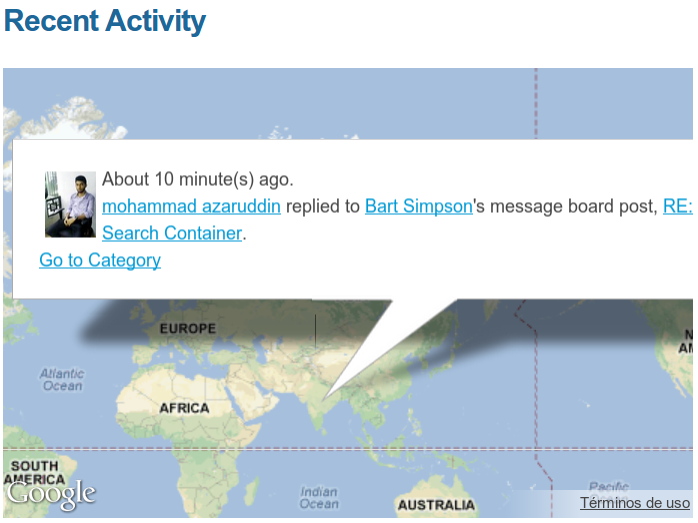
\includegraphics{http://2.bp.blogspot.com/-8ssRjUhvKvY/UVAoIkVI5GI/AAAAAAAAEKU/xGQoWq1NUUg/s640/liferay-dashboard.png}} \\ 
Liferay Contributions Dashboard
\end{tabular} Our firs impresion is that Liferay community is developed worldwide. They publish community analysis, workshops, releases and community success samples.
\\ It's important to start reading\nolinebreak\href{http://www.liferay.com/documentation/liferay-portal/6.1/user-guide}{Liferay user guide}, everyone should start from here, because you need to know first what Liferay is.
\\ Liferay encourages users to create a profile page, as we can se \href{http://www.liferay.com/web/jorge.ferrer/profile}{Jorge Ferrer Liferay} personal page. Gives importance to create a 'centralized' community.
\\ Like other FLOSS projects they divide community section in two main groups:
\begin{itemize}
	\item Participate -\nolinebreak\href{http://www.liferay.com/community/welcome/participate}{http://www.liferay.com/community/welcome/participate}
	\item Contribute -\nolinebreak\href{http://www.liferay.com/community/welcome/contribute}{http://www.liferay.com/community/welcome/contribute}
\end{itemize}\textit{Participate} section invites the user to share the experience of liferay, doubts, achievements, proposals, errors found, so that people who encounter the same mistakes do not recur. Thus, creating a place to clarify questions and share knowledge, Liferay community.
\\ You can find different ways to communicate with Liferay community, \textit{communicate is as valuable as contribute with code}:
\begin{itemize}
	\item Community Forum
	\item Blogs
	\item Wiki
	\item IRC
	\item Liferay LIVE
	\item Events
	\item Issues
	\item User Groups
\end{itemize} In \textit{Contribute} section you have more technical information about how to contribute 'explicit' with communty. \href{http://www.liferay.com/community/wiki/-/wiki/Main/Contributing}{Wiki section} explains different ways and each guide defined to contribute. There is a wide fork to contribute, from translations to writing a complete Liferay plugin:
\begin{itemize}
	\item \textit{Reporting and/or fixing a bug}: \href{http://issues.liferay.com/secure/Dashboard.jspa}{JIRA ITS} is used to provide easy bug/issueTS interface for users. Explained detailed how to report a bug, publish it, search for it and develop a solution.
	\item \href{http://www.liferay.com/community/wiki/-/wiki/Main/Contributing#section-Contributing-Write+documentation}{\textit{Writing documentation}}: In Wiki section is described that every user can write Liferay documentaiton. There are two main guides \textit{Wiki Guidelines} and\nolinebreak\textit{Liferay Editorial Guidelines}\nolinebreakto contribute with documentation.
	\item \textit{Implementing a new feature}: Section \href{http://www.liferay.com/community/wiki?p_p_id=36&amp;p_p_lifecycle=0&amp;p_p_state=normal&amp;p_p_mode=view&amp;p_p_col_id=column-2&amp;p_p_col_count=1&amp;_36_struts_action=%2Fwiki%2Fedit_page&amp;_36_redirect=http%3A%2F%2Fwww.liferay.com%2Fcommunity%2Fwiki%2F-%2Fwiki%2FMain%2FHow%2Bto%2Bcontribute%2Bto%2BLiferay&amp;p_r_p_185834411_nodeId=1071674&amp;p_r_p_185834411_title=Proposed+Projects}{Proposed Projects}\nolinebreakto describe your solution after read and develop your new feature described in \href{http://www.liferay.com/community/wiki/-/wiki/Main/Liferay+Core+Development+Guidelines}{trunk Development Guidelines}. Also you can suggest a new feature in \href{http://www.liferay.com/web/guest/community/forums/-/message_boards/category/1108052}{Liferay Forum}.
	\item \textit{Providing Translations}: Liferay \href{http://www.liferay.com/community/wiki/-/wiki/Main/Translation+Team}{Translation Team}\nolinebreakhas its own guidelines to manage translation teams for each Language.
	\item \textit{Writing a useful plugin}: They provide a complete developers guide for Liferay plugins in pdf. You can download it \href{http://docs.liferay.com/portal/6.0/official/liferay-developer-guide-6.0.pdf}{here}.
\end{itemize} Ohter remarcable section is \href{http://www.liferay.com/community/ideas}{Community Feature Ideas}. The user can provide ideas to Liferay evolution. Manages JIRA to advertise for Liferay different ideas,\nolinebreak\nolinebreakJIRA\nolinebreakbecomes more social and guided by the votes of the people to develop new ideas.

\subsubsection{ Technologies} Liferay is delevoped in Java and uses \href{http://sourceforge.net/projects/lportal/files/Liferay%20IDE/1.4.0/liferay-ide-eclipse-updatesite-1.4.0.zip/download}{Eclipse Liferay IDE for developers}. Also needs Liferay Portals and SDK to start developing. With this complete pack you can start developing your own portlets, themes and extensions for Liferay.
\\ There is a guide to develop \href{http://www.liferay.com/community/wiki/-/wiki/Main/Liferay+6.0+Development+on+Ubuntu+Maverick+10.10}{Liferay in Ubuntu}\nolinebreakexplaining from installation to deployment process.
\\ Liferay uses Git and has GitHub profile -\nolinebreak\href{https://github.com/liferay}{https://github.com/liferay}. They use GitHub as code reviewer tool linked with JIRA issues and Forum questions.
\\ So, here is the picture:
\begin{itemize}
	\item Read Documentation guidelines.
	\item Install Liferay Development Environment.
	\item Search for an Issue.
	\item Develop a solution using guidelines.
	\item Make a \textit{pull request} from GitHub to review code.
\end{itemize} Technologies used in contribution process are: \textit{Java, Eclipse, Git, GitHub, Forum and JIRA}. I encourage you to take a tour in next (work in progress) Liferay Development, \textit{\href{http://www.liferay.com/es/documentation/liferay-portal/6.1/user-guide/-/ai/osgi}{OSGI Migration Documentation}.}